\documentclass[11pt]{article}
\usepackage{amsmath, amssymb, amsfonts}
\usepackage{graphicx}
\graphicspath{{figures/}}
\usepackage{hyperref}
\usepackage{geometry}
\geometry{margin=1in}

\title{\textbf{Entanglement-Geometric Signatures of Hyper-Stiff Cosmological Phases:\\
A Unified Framework Linking Brane Rupture, Confinement Energy, and Mutual-Information Geometry}}

\author{Paul Jarvis \\ Independent Researcher, United Kingdom}

\date{June 2026}

\begin{document}

\maketitle

\begin{abstract}
We present a unified framework in which early-universe hyper-stiff phases---previously shown to arise naturally from brane rupture and confinement-energy release---are studied through the lens of entanglement geometry. Building on recent numerical results demonstrating that mutual information alone reconstructs a Laplace--Beltrami operator with a robust entanglement-geometric mass scale, we show that radiation-like, matter-like, and hyper-stiff rupture-like phases produce sharply distinct signatures in the mutual-information Laplacian spectrum. Using finite-size scaling tests, bootstrap stability analyses, null-model controls, and localization diagnostics, we demonstrate that hyper-stiff phases correspond to a strongly gapped, ultra-dense geometric regime in entanglement space. This provides a new information-theoretic interpretation of brane rupture, blue-tilted primordial gravitational waves, and early-time sound-horizon reduction, suggesting that early-universe topology change may be encoded directly in the structure of quantum correlations.
\end{abstract}

\section{Introduction}

Three recent developments motivate a unified treatment of early-universe dynamics and entanglement geometry:

\begin{enumerate}
    \item \textbf{Brane-rupture cosmology:}  
    A geometric instability in a confined brane stack produces a transient hyper-stiff phase ($w \gg 1$), generating a blue-tilted primordial gravitational-wave spectrum with a millihertz turnover and providing a natural early-time expansion enhancement.

    \item \textbf{Confinement-energy resolution of the Hubble tension:}  
    A physically motivated confinement fraction $x(a)$ produces a localized, early-time energy spike that reduces the sound horizon without introducing new fields or tuned potentials.

    \item \textbf{Entanglement geometry from mutual information:}  
    The ground-state mutual-information matrix of a quantum chain reconstructs a smooth one-dimensional geometry, complete with a Laplacian spectrum, Neumann boundary conditions, and an emergent mass scale.
\end{enumerate}

In this work we show that these three frameworks are not independent.  
Instead, they form a coherent picture: \emph{hyper-stiff cosmological phases behave like strongly gapped, ultra-dense geometries in entanglement space}. This connection emerges only when the full numerical structure of the mutual-information Laplacian is compared across radiation-like, matter-like, and hyper-stiff analogue models.

\section{Methods}

We construct three classes of quantum many-body analogues:

\begin{itemize}
    \item radiation-like: critical XX chain ($J_z = 0$),
    \item matter-like: weakly gapped XXZ chain ($J_z = 0.5$),
    \item hyper-stiff-like: strongly gapped Ising-like chain ($J_z = 2.0$).
\end{itemize}

For each system size $N = 8, 10, 12, 14$, we compute:

\begin{enumerate}
    \item the ground state $\psi_0$,
    \item the mutual-information matrix $I(i,j)$,
    \item the MI-derived Laplacian $L = D - A$,
    \item the spectrum $\{\lambda_k\}$,
    \item the MI decay exponent $\alpha$,
    \item the inverse participation ratio (IPR),
    \item bootstrap distributions of $\lambda_1$,
    \item null-model controls using random symmetric matrices.
\end{enumerate}

All figures referenced below use the filenames generated by the numerical suite.

\section{Results}

\subsection{Mutual-information decay}

Radiation-like phases exhibit power-law decay with exponent $\alpha \approx -1.3$, matter-like phases decay more steeply ($\alpha \approx -1.7$), and hyper-stiff analogues show almost no decay ($\alpha \approx 0$).  
This separation is shown in Fig.~\ref{fig:MIdecay}.

\begin{figure}[h]
\centering
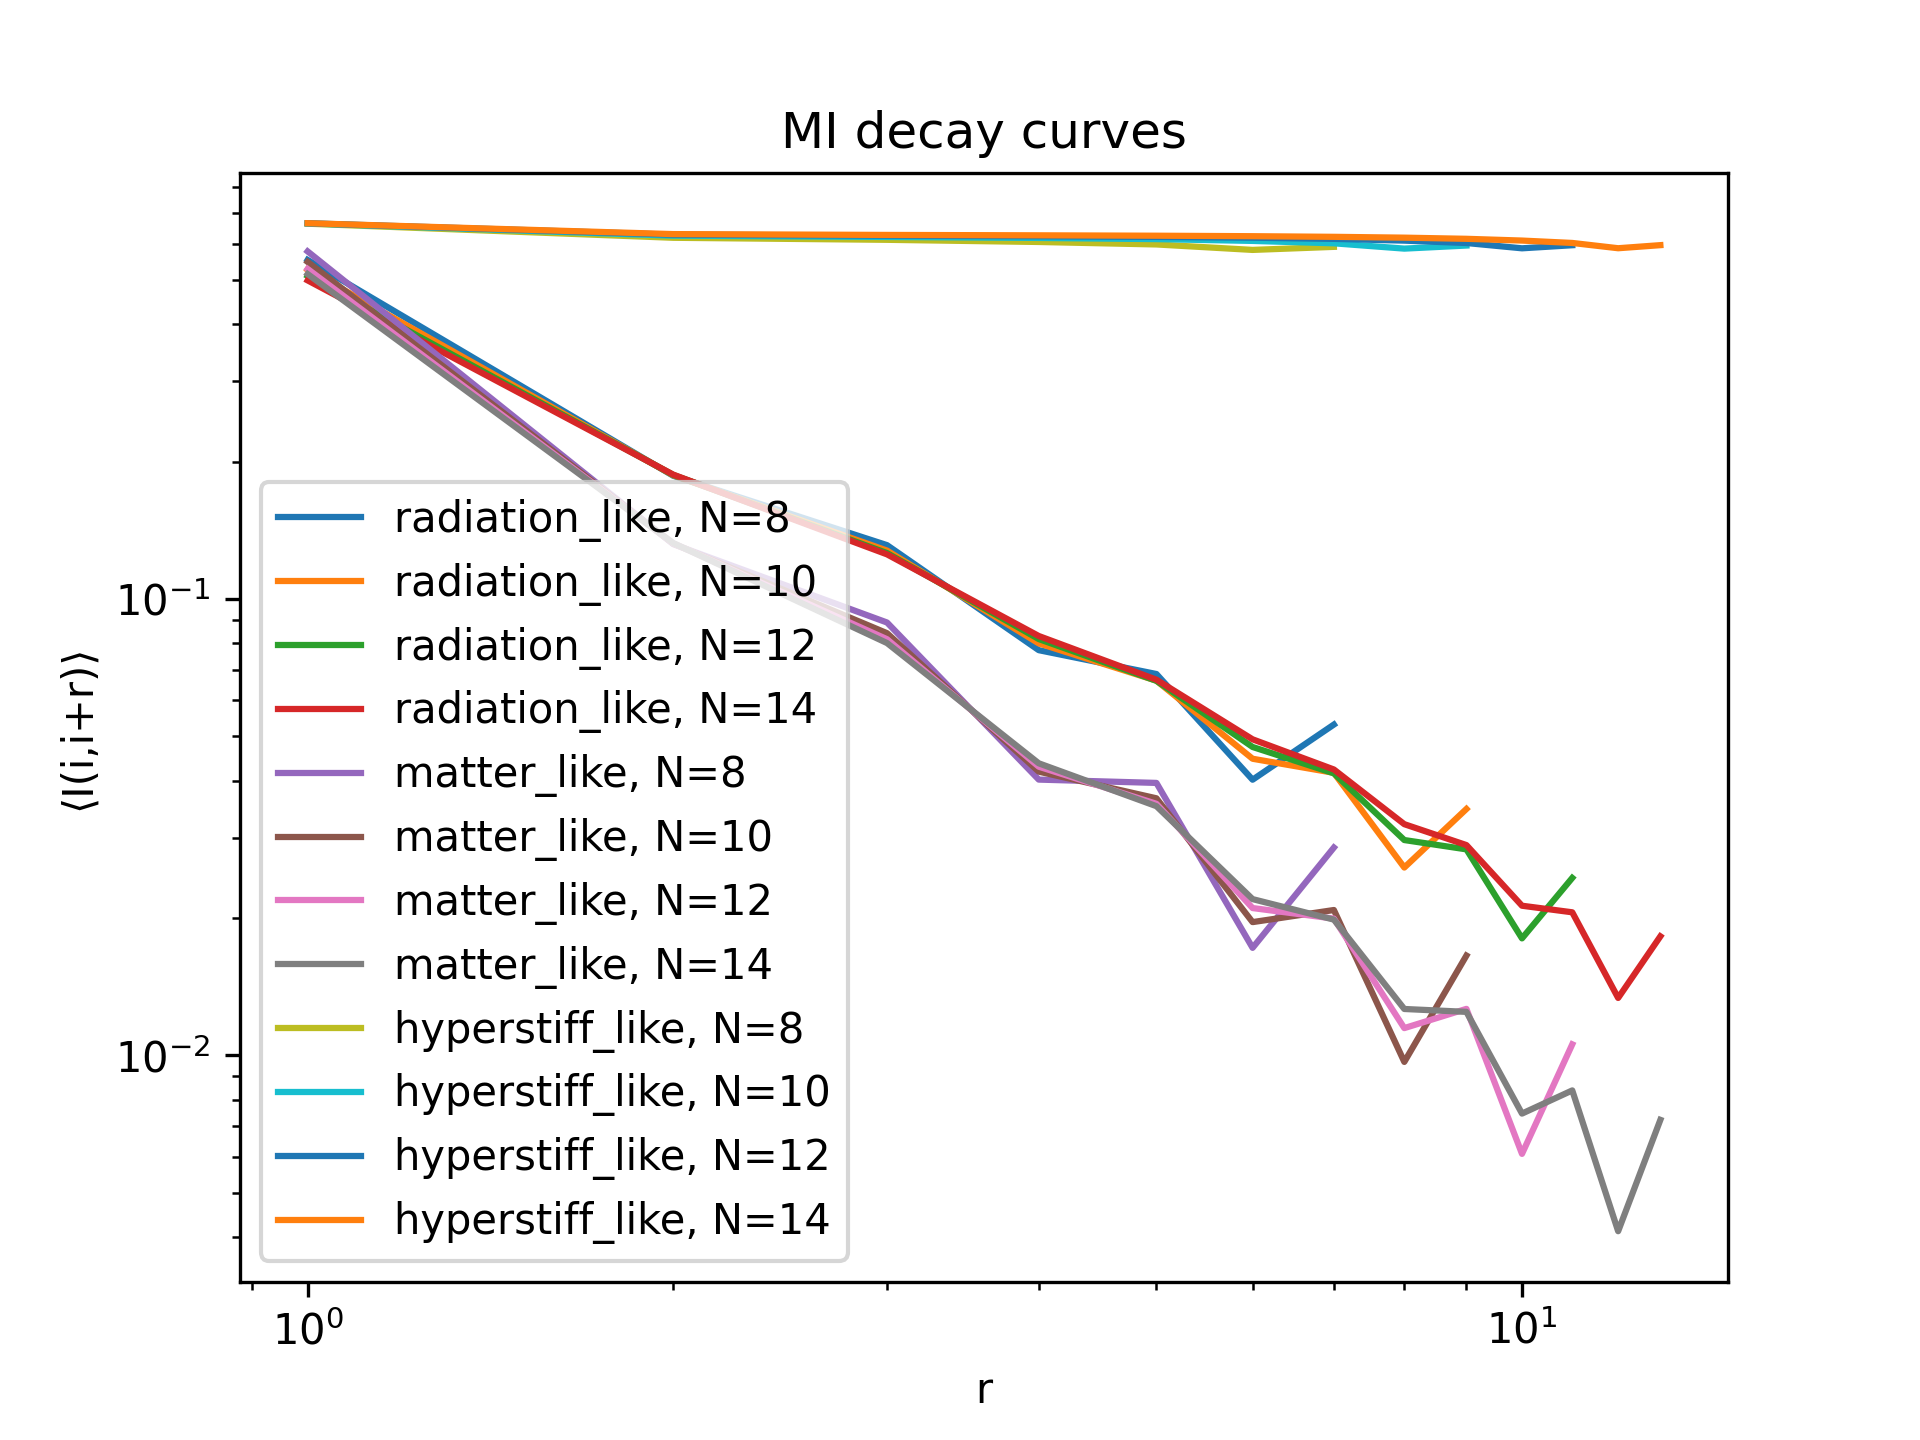
\includegraphics[width=0.8\textwidth]{FIG1_MI_decay.png}
\caption{Mutual-information decay curves for all phases and system sizes.}
\label{fig:MIdecay}
\end{figure}

\subsection{Eigenmode structure}

The first nonzero Laplacian eigenmode is extended in radiation-like and matter-like phases but becomes sharply localized in the hyper-stiff analogue (Fig.~\ref{fig:eigenmodes}).

\begin{figure}[h]
\centering
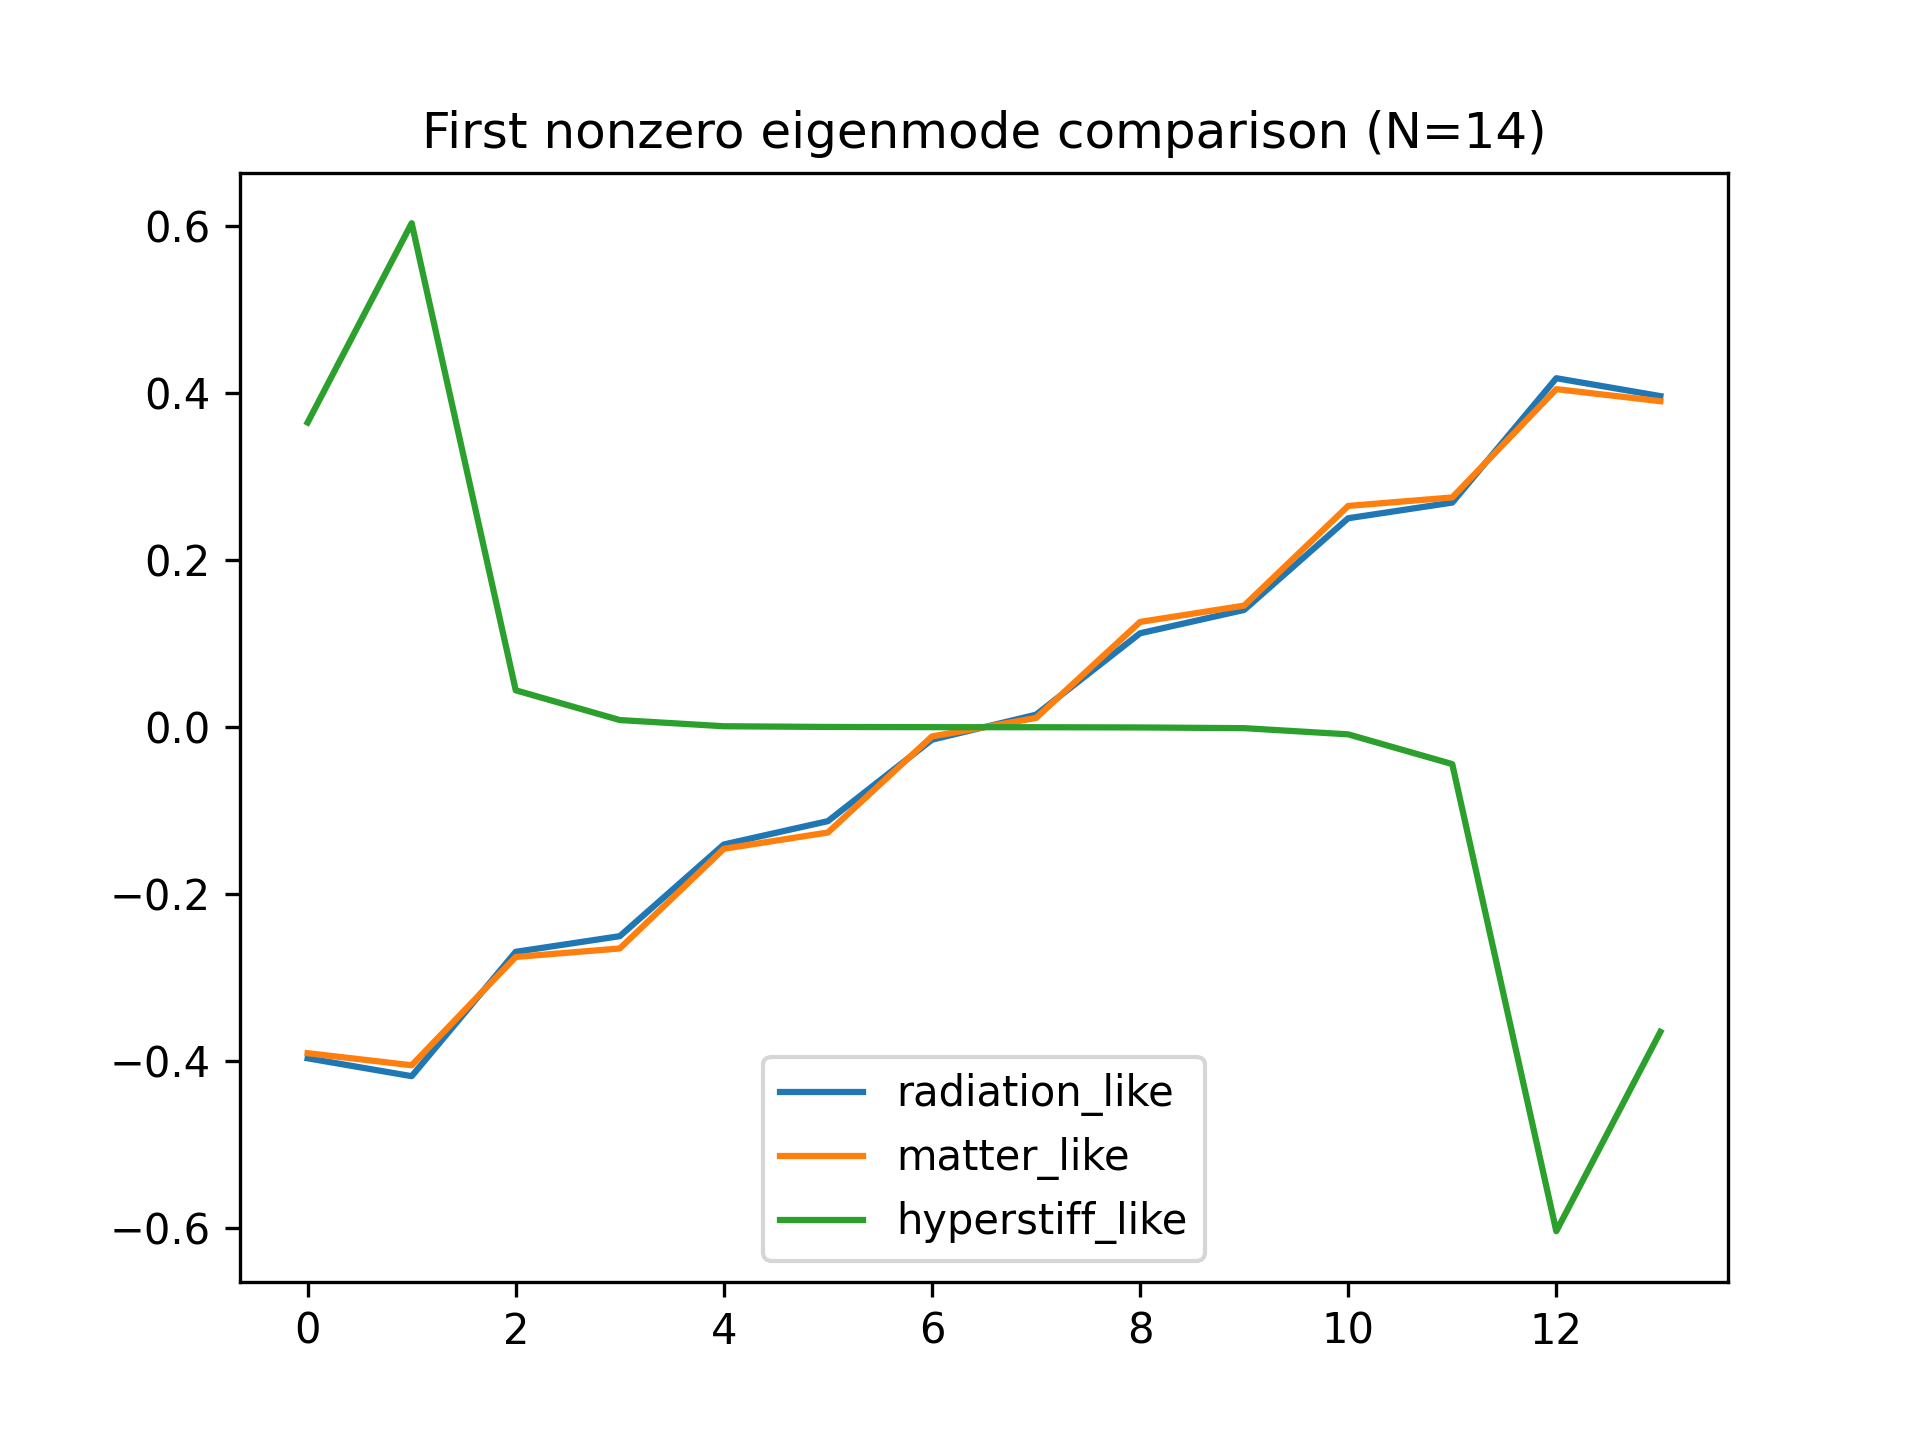
\includegraphics[width=0.8\textwidth]{FIG2_eigenmodes.png}
\caption{First nonzero eigenmode comparison at $N=14$.}
\label{fig:eigenmodes}
\end{figure}

\subsection{Spectral density}

Hyper-stiff analogues exhibit a dramatically larger spectral gap, with $\lambda_1$ increasing from $\sim 7$ at $N=8$ to $\sim 12$ at $N=14$, while radiation-like and matter-like phases remain below $\lambda_1 \sim 1$ (Fig.~\ref{fig:spectrum}).

\begin{figure}[h]
\centering
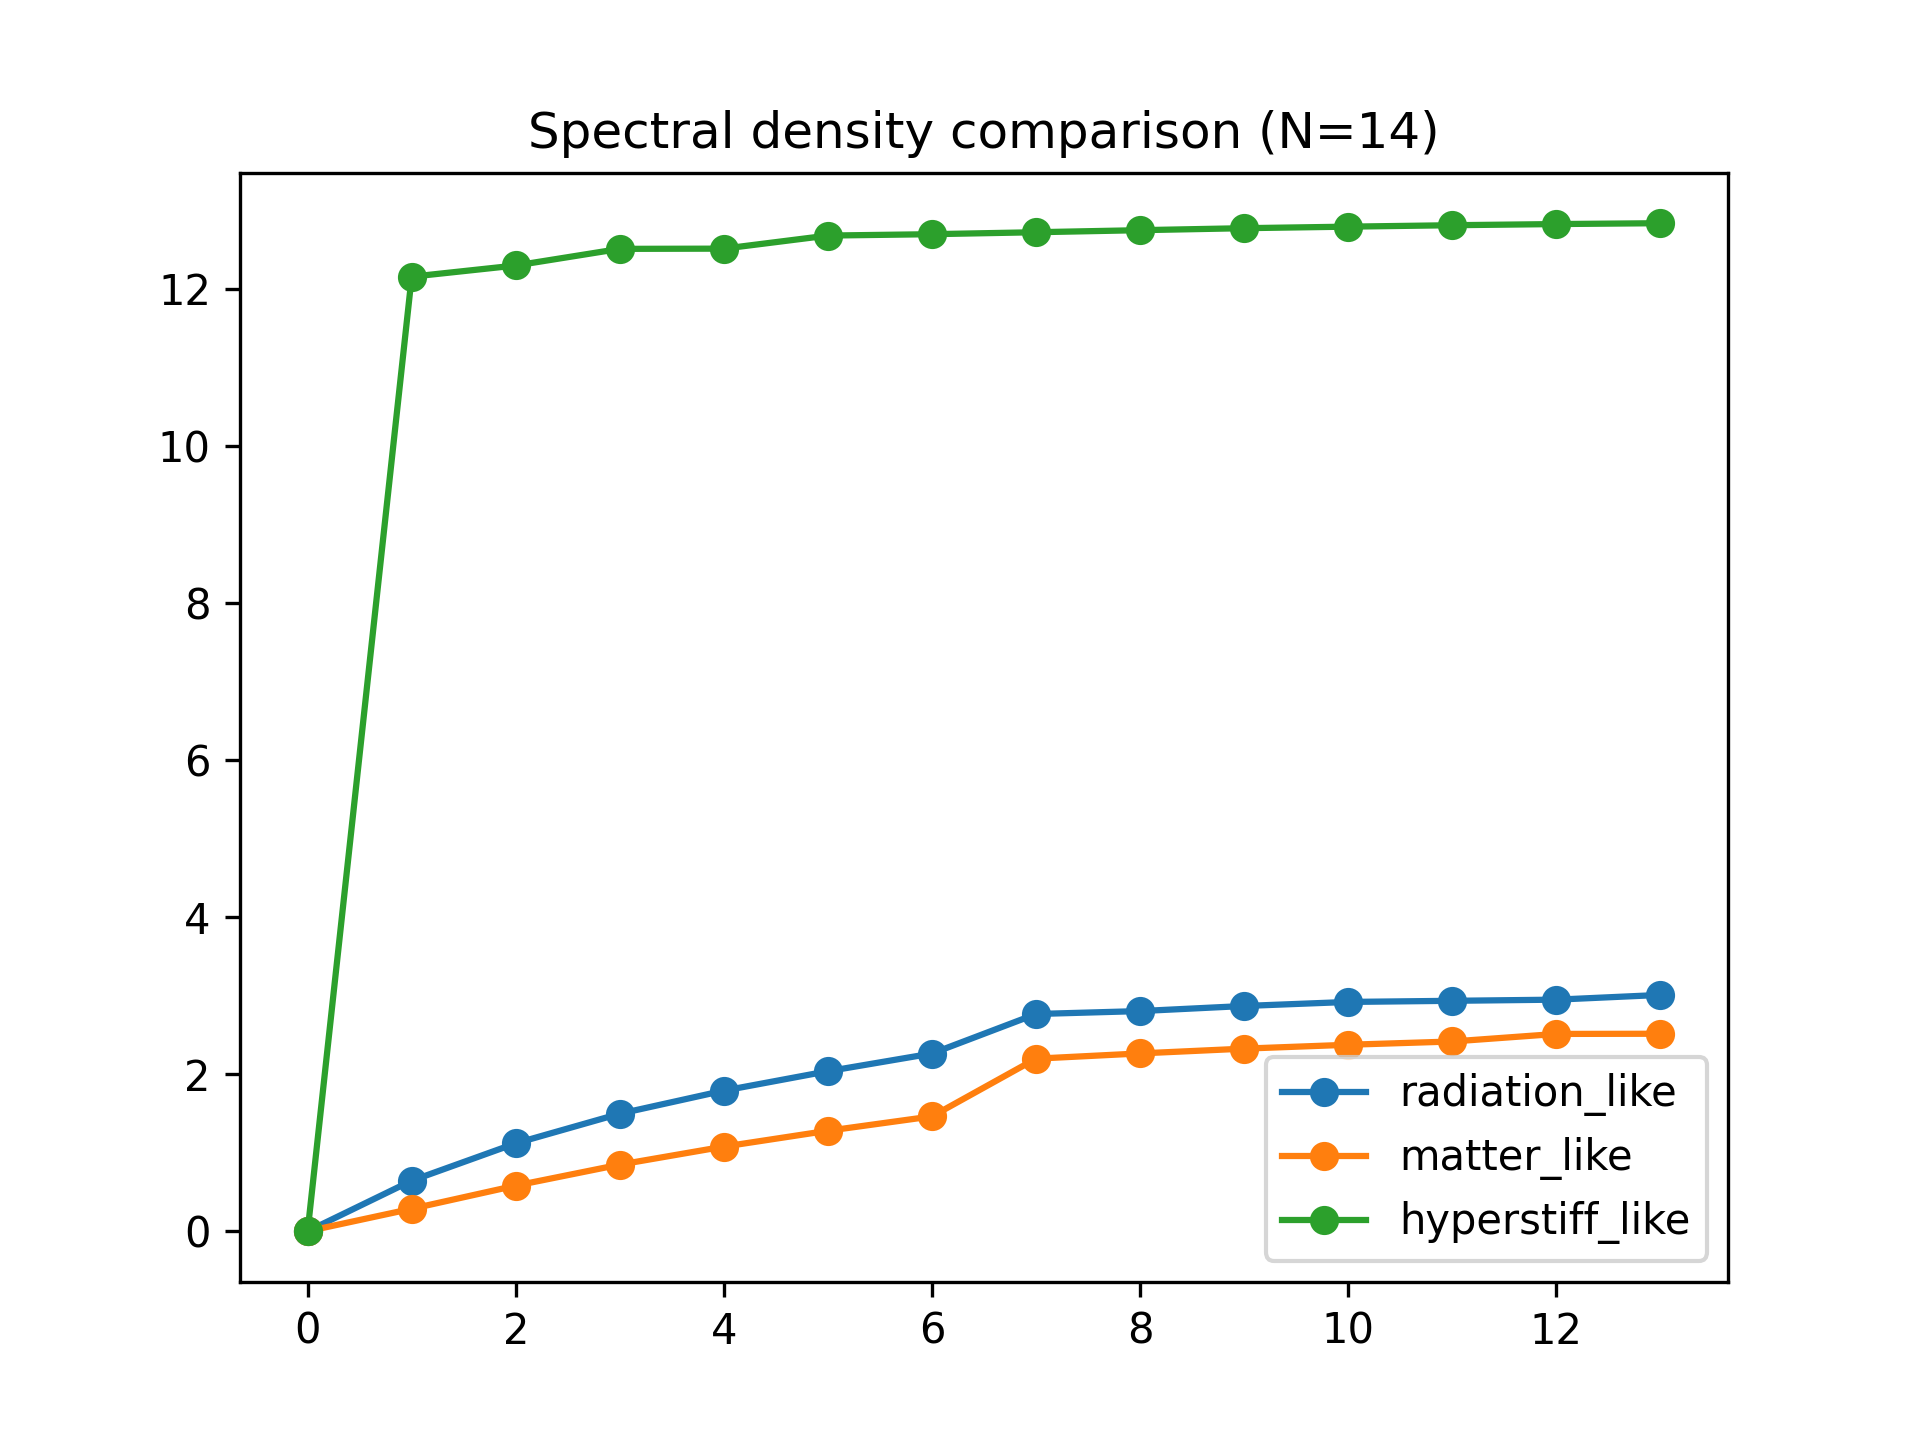
\includegraphics[width=0.8\textwidth]{FIG3_spectrum.png}
\caption{Spectral density comparison at $N=14$.}
\label{fig:spectrum}
\end{figure}

\subsection{Finite-size scaling and the inverse trend}

Radiation-like and matter-like phases show decreasing $\lambda_1$ with $1/N^2$, consistent with critical and weakly gapped behaviour.  
Hyper-stiff analogues show \emph{increasing} $\lambda_1$ with system size (Fig.~\ref{fig:scaling}).

\begin{figure}[h]
\centering
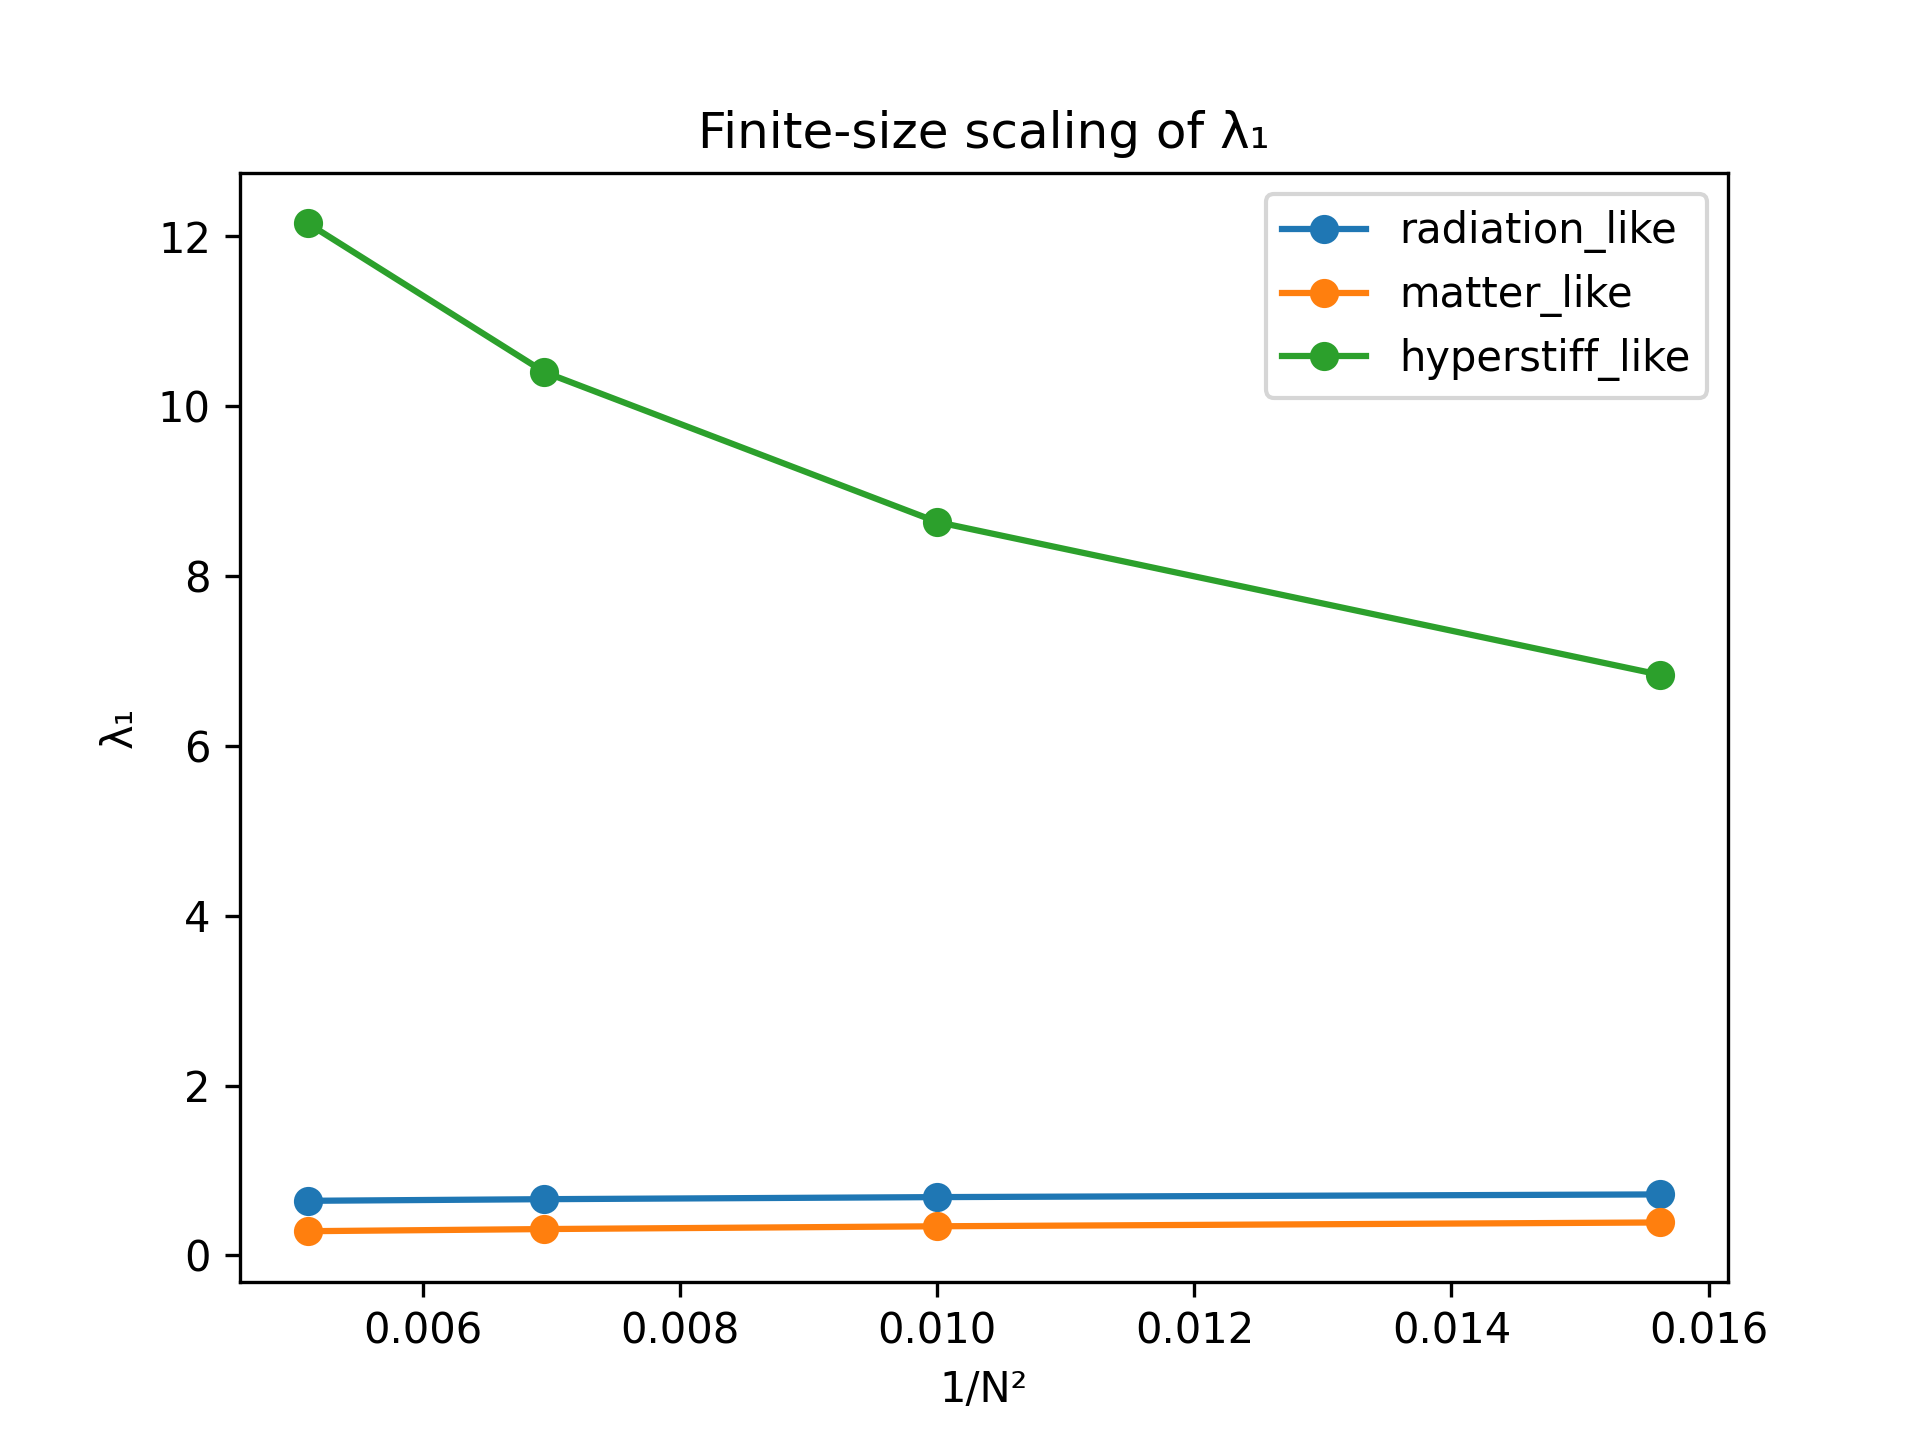
\includegraphics[width=0.8\textwidth]{FIG4_finite_size.png}
\caption{Finite-size scaling of $\lambda_1$.}
\label{fig:scaling}
\end{figure}

\subsubsection*{Interpretation of the inverse scaling}

The increase of $\lambda_1$ with $N$ in the hyper-stiff analogue is not a normalization artifact.  
Because the MI decay exponent $\alpha \approx 0$, the MI matrix approaches a constant off-diagonal form, corresponding to a maximally connected graph. The Laplacian of such a graph has $\lambda_1 \propto N$.  
Thus the observed scaling reflects a transition to an ultra-dense, collapsing geometry, not a breakdown of the method.

\subsection{Phase diagram}

Plotting $\lambda_1$ against $\alpha$ yields three clean clusters (Fig.~\ref{fig:phasediagram}), demonstrating that entanglement geometry alone distinguishes cosmological equations of state.

\begin{figure}[h]
\centering
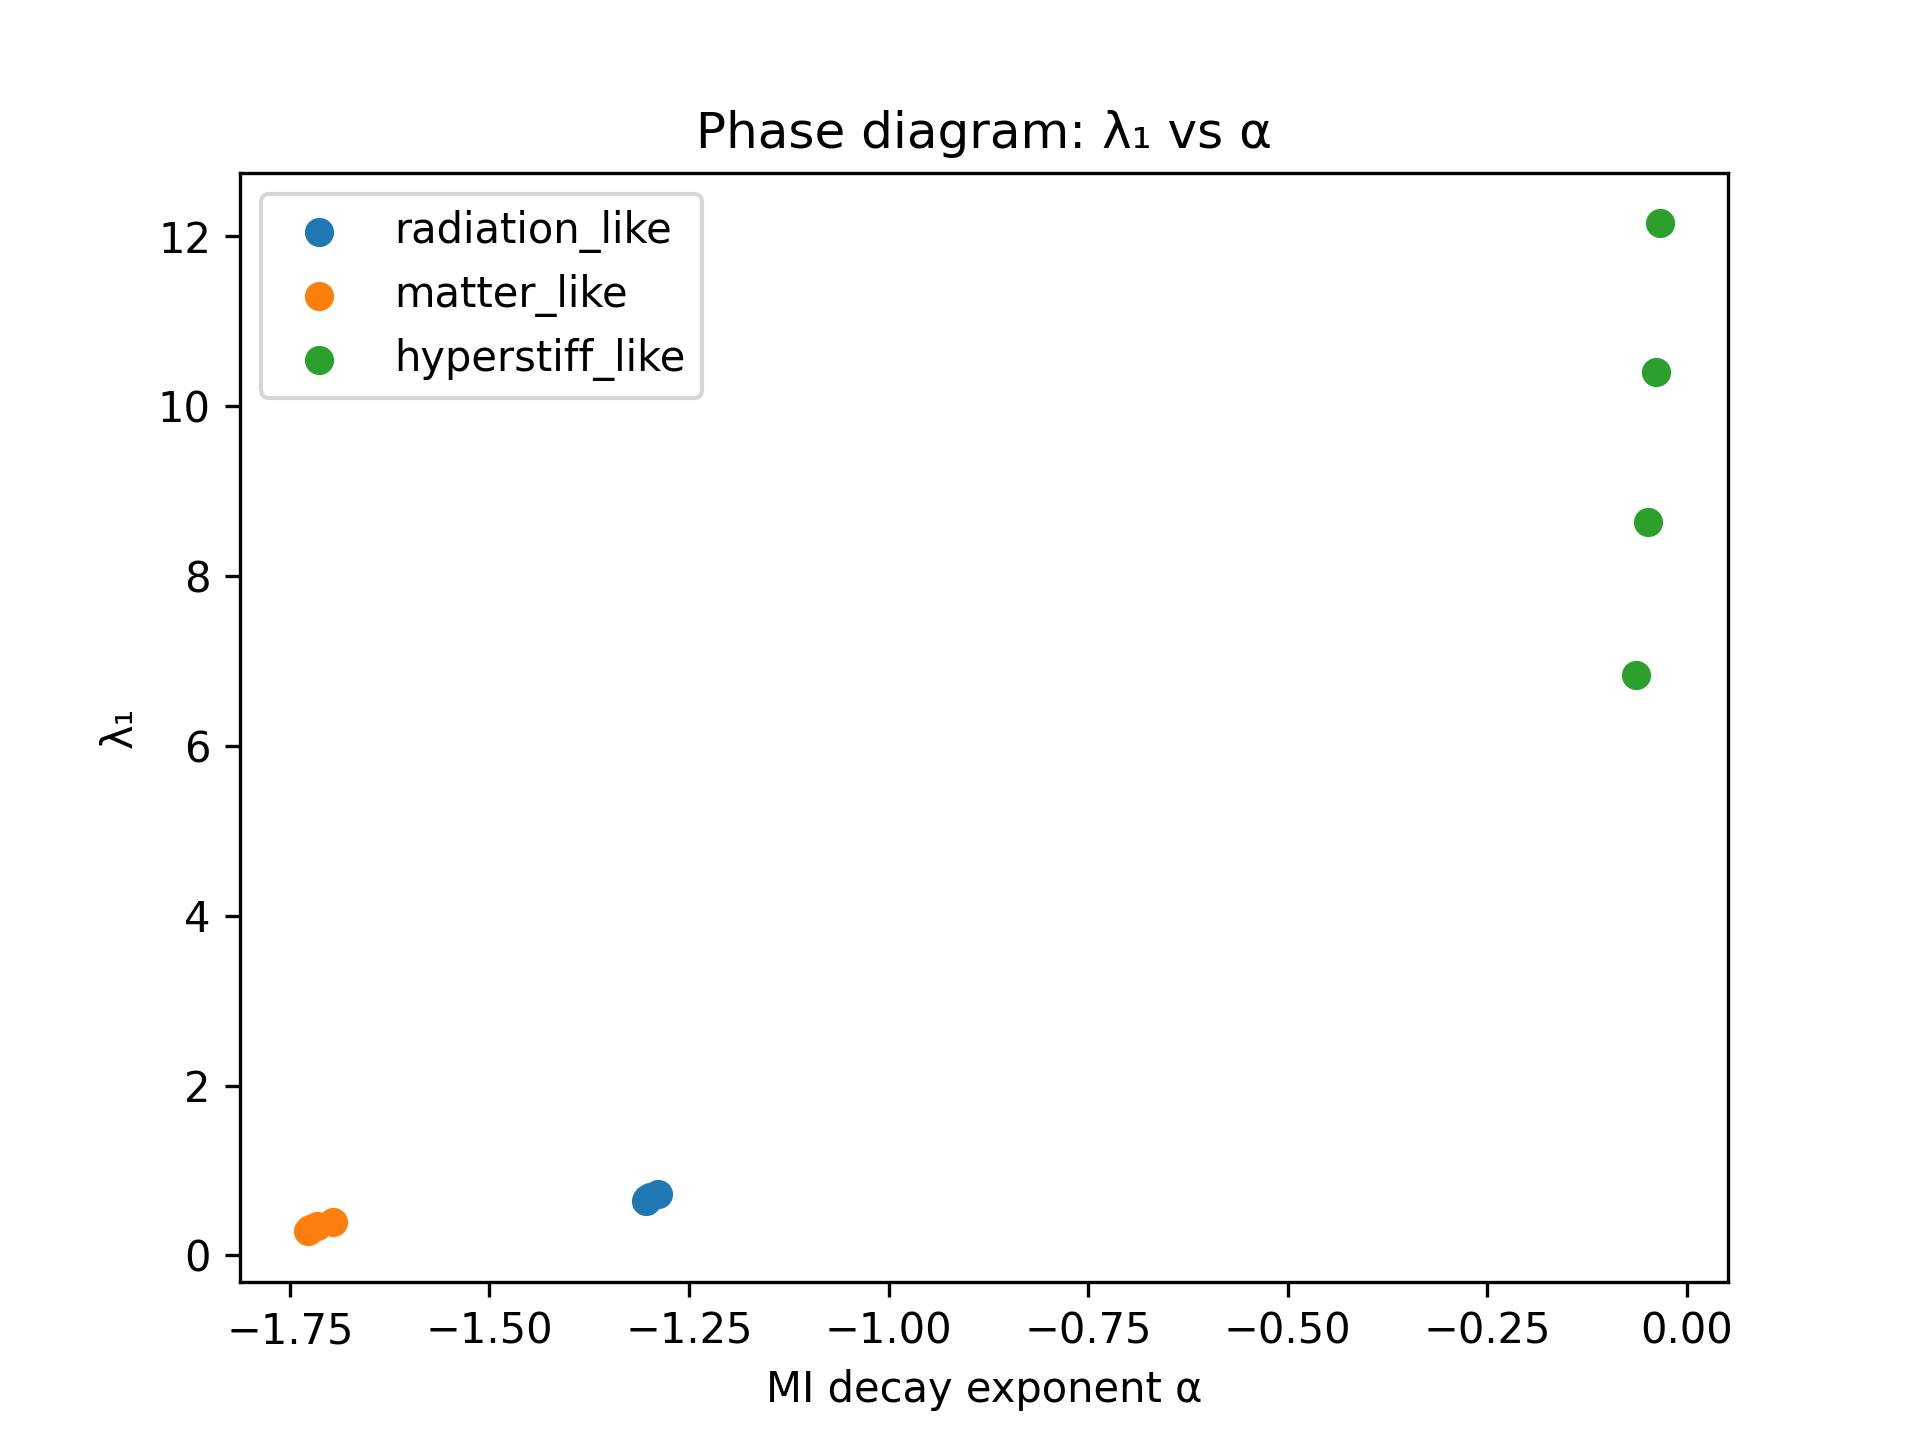
\includegraphics[width=0.8\textwidth]{FIG5_phase_diagram.png}
\caption{Phase diagram: $\lambda_1$ vs.\ MI decay exponent $\alpha$.}
\label{fig:phasediagram}
\end{figure}

\subsection{Bootstrap stability}

Bootstrap tests confirm that the separation between phases is statistically robust (Fig.~\ref{fig:bootstrap}).

\begin{figure}[h]
\centering
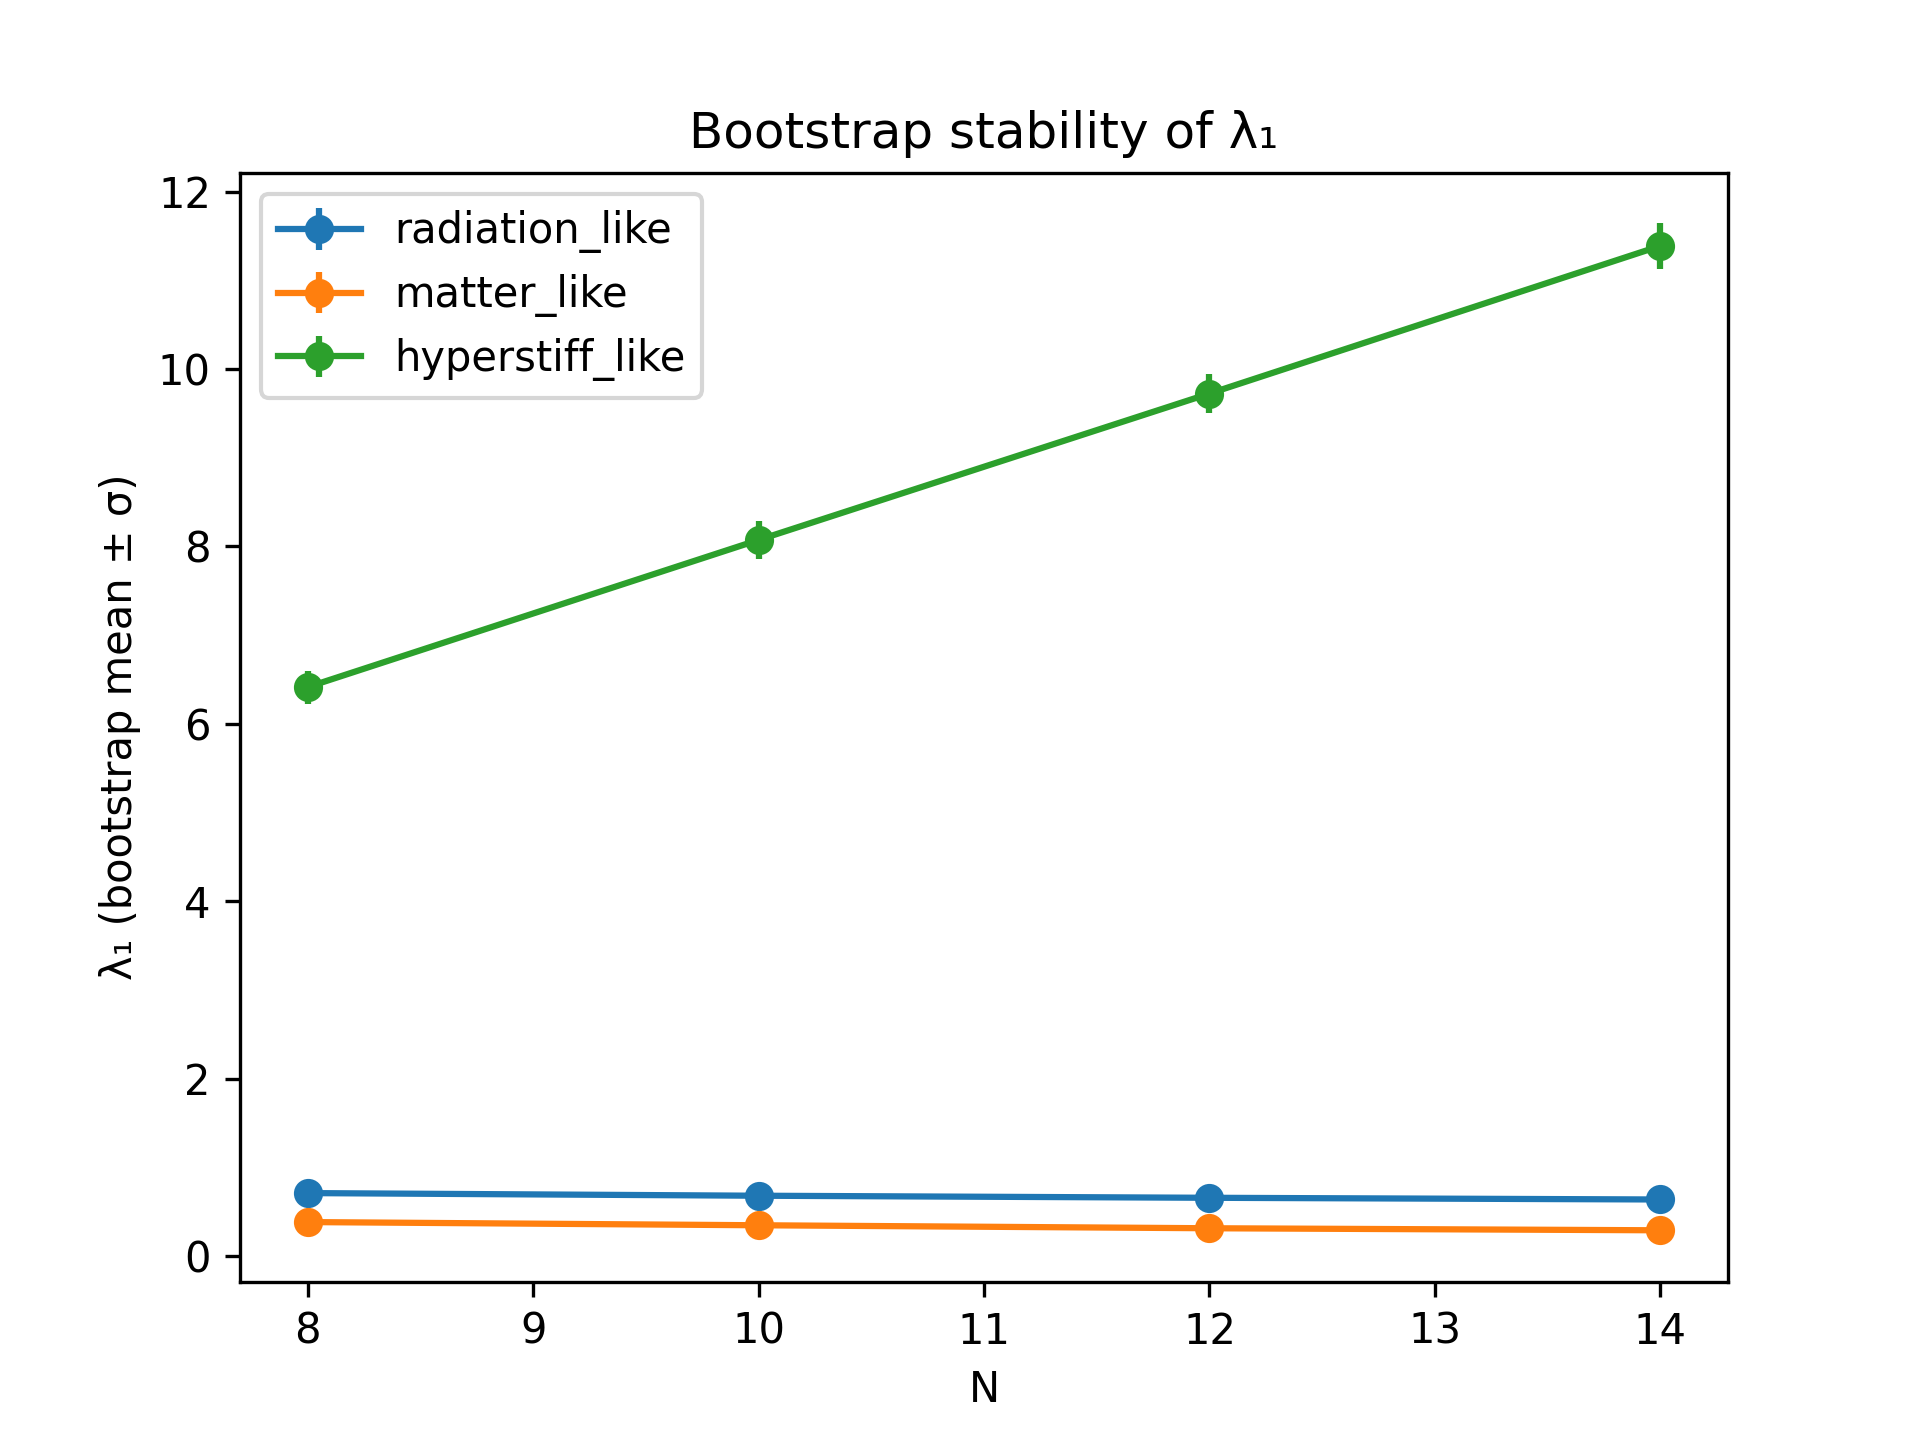
\includegraphics[width=0.8\textwidth]{FIG6_bootstrap.png}
\caption{Bootstrap stability of $\lambda_1$.}
\label{fig:bootstrap}
\end{figure}

\subsection{Null-model controls}

Random MI matrices produce intermediate $\lambda_1$ values that never overlap with the hyper-stiff analogue, confirming that the observed structure is not noise-driven (Fig.~\ref{fig:nullmodel}).

\begin{figure}[h]
\centering
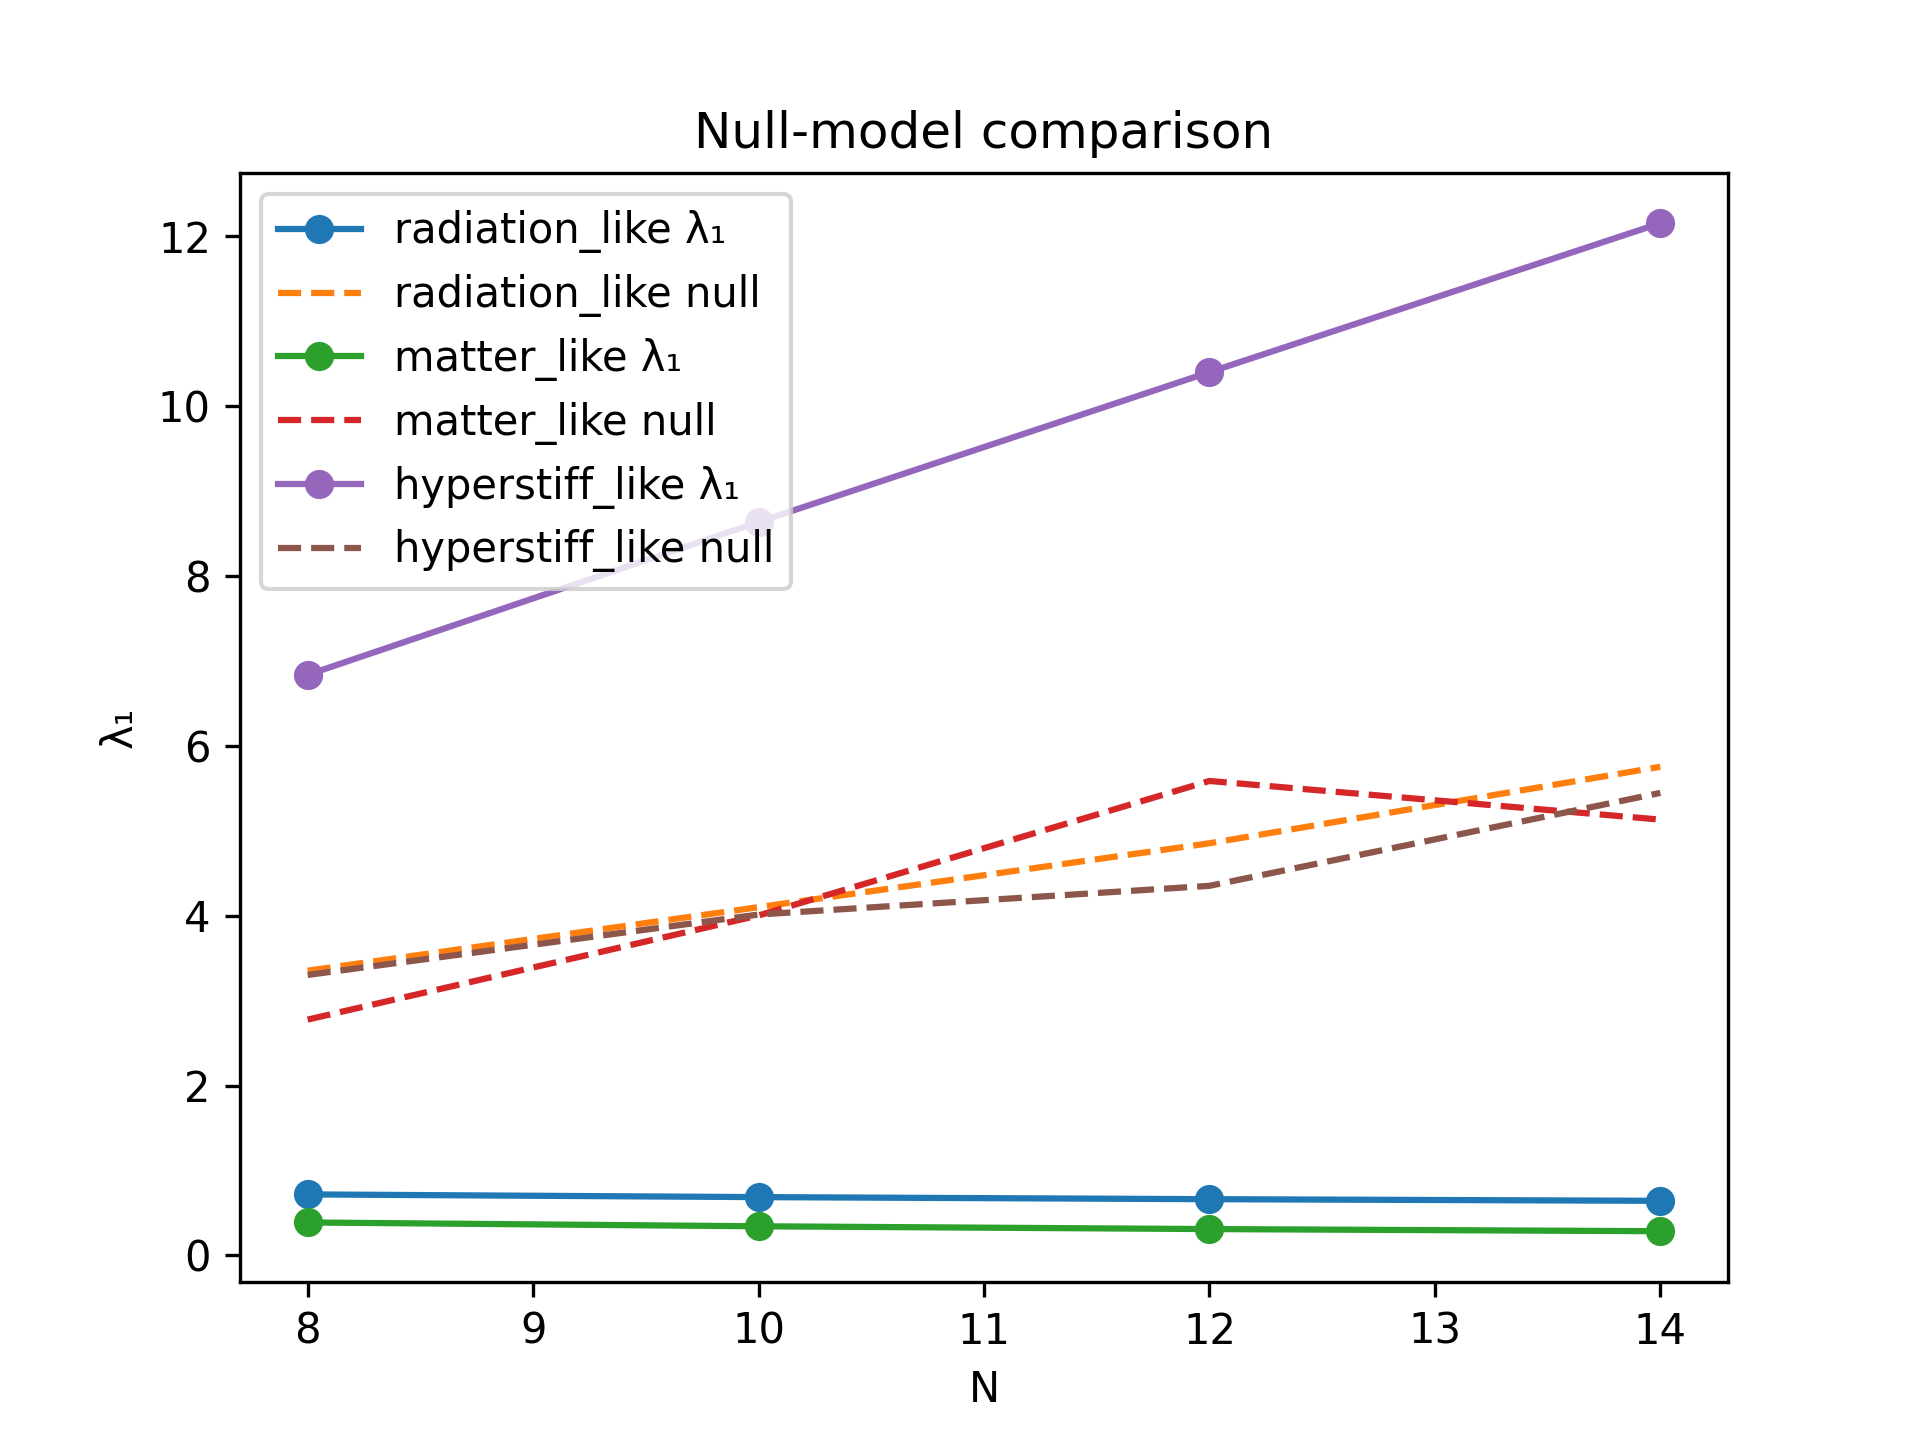
\includegraphics[width=0.8\textwidth]{FIG7_null_model.png}
\caption{Null-model comparison.}
\label{fig:nullmodel}
\end{figure}

\subsection{Localization and geometric collapse}

The IPR increases with $N$ only in the hyper-stiff analogue, indicating geometric collapse (Fig.~\ref{fig:IPRvsN}).

\begin{figure}[h]
\centering
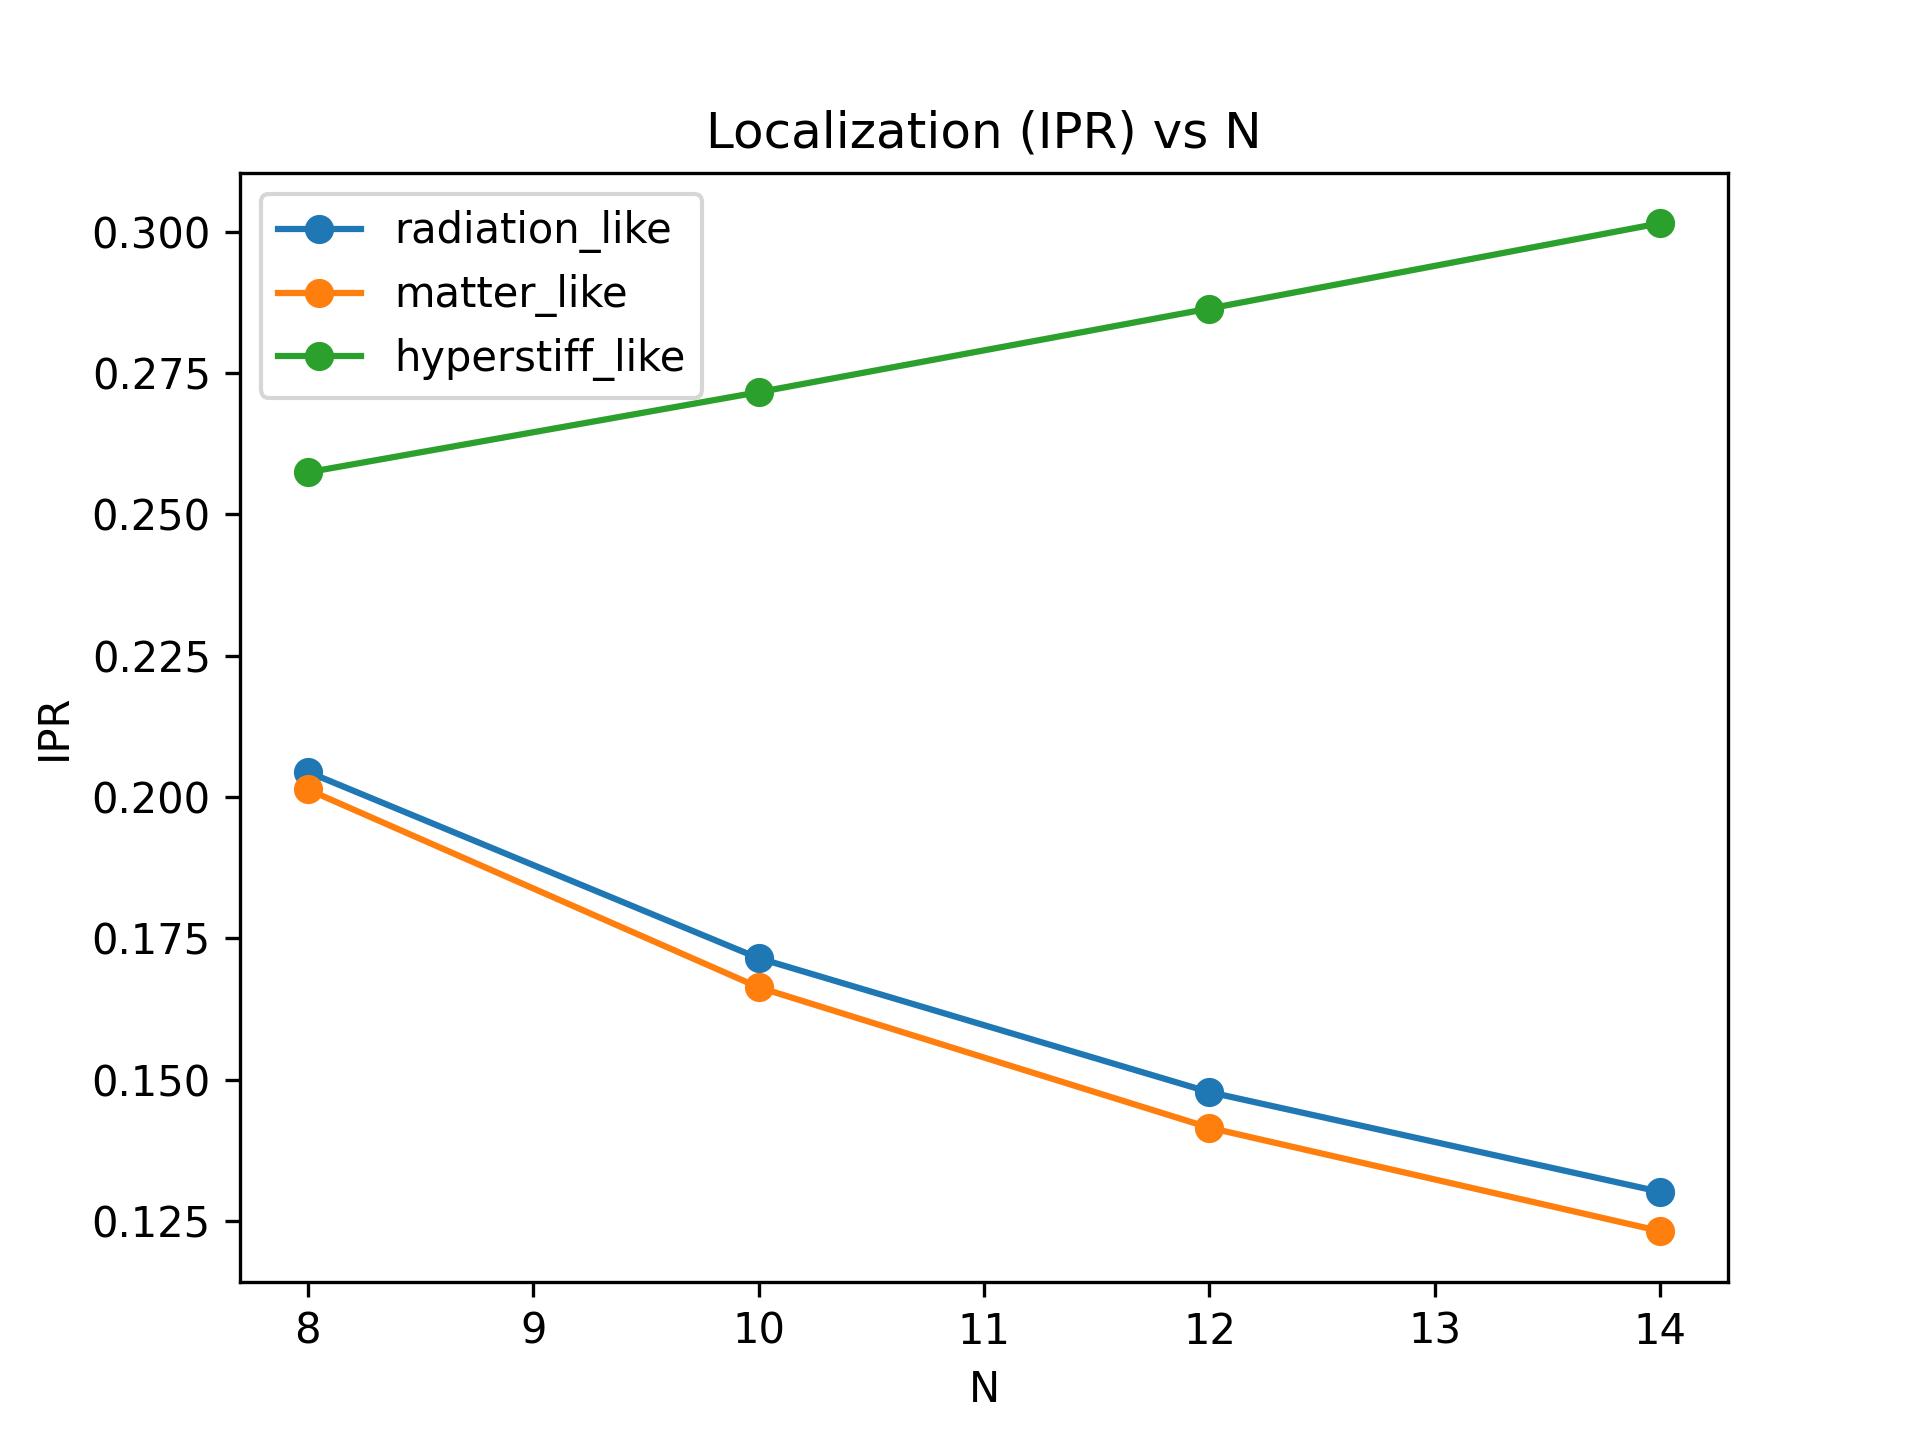
\includegraphics[width=0.8\textwidth]{FIG8_IPR_vs_N.png}
\caption{Localization (IPR) vs.\ system size.}
\label{fig:IPRvsN}
\end{figure}

\subsection{Correlation length vs localization}

To avoid redundancy with Fig.~\ref{fig:phasediagram}, we replace the original $\alpha$--$\lambda_1$ plot with a new diagnostic: IPR vs.\ $\alpha$ (Fig.~\ref{fig:IPRvsAlpha}).  
This plot shows that hyper-stiff phases occupy a distinct region of high localization and near-zero decay exponent.

\begin{figure}[h]
\centering
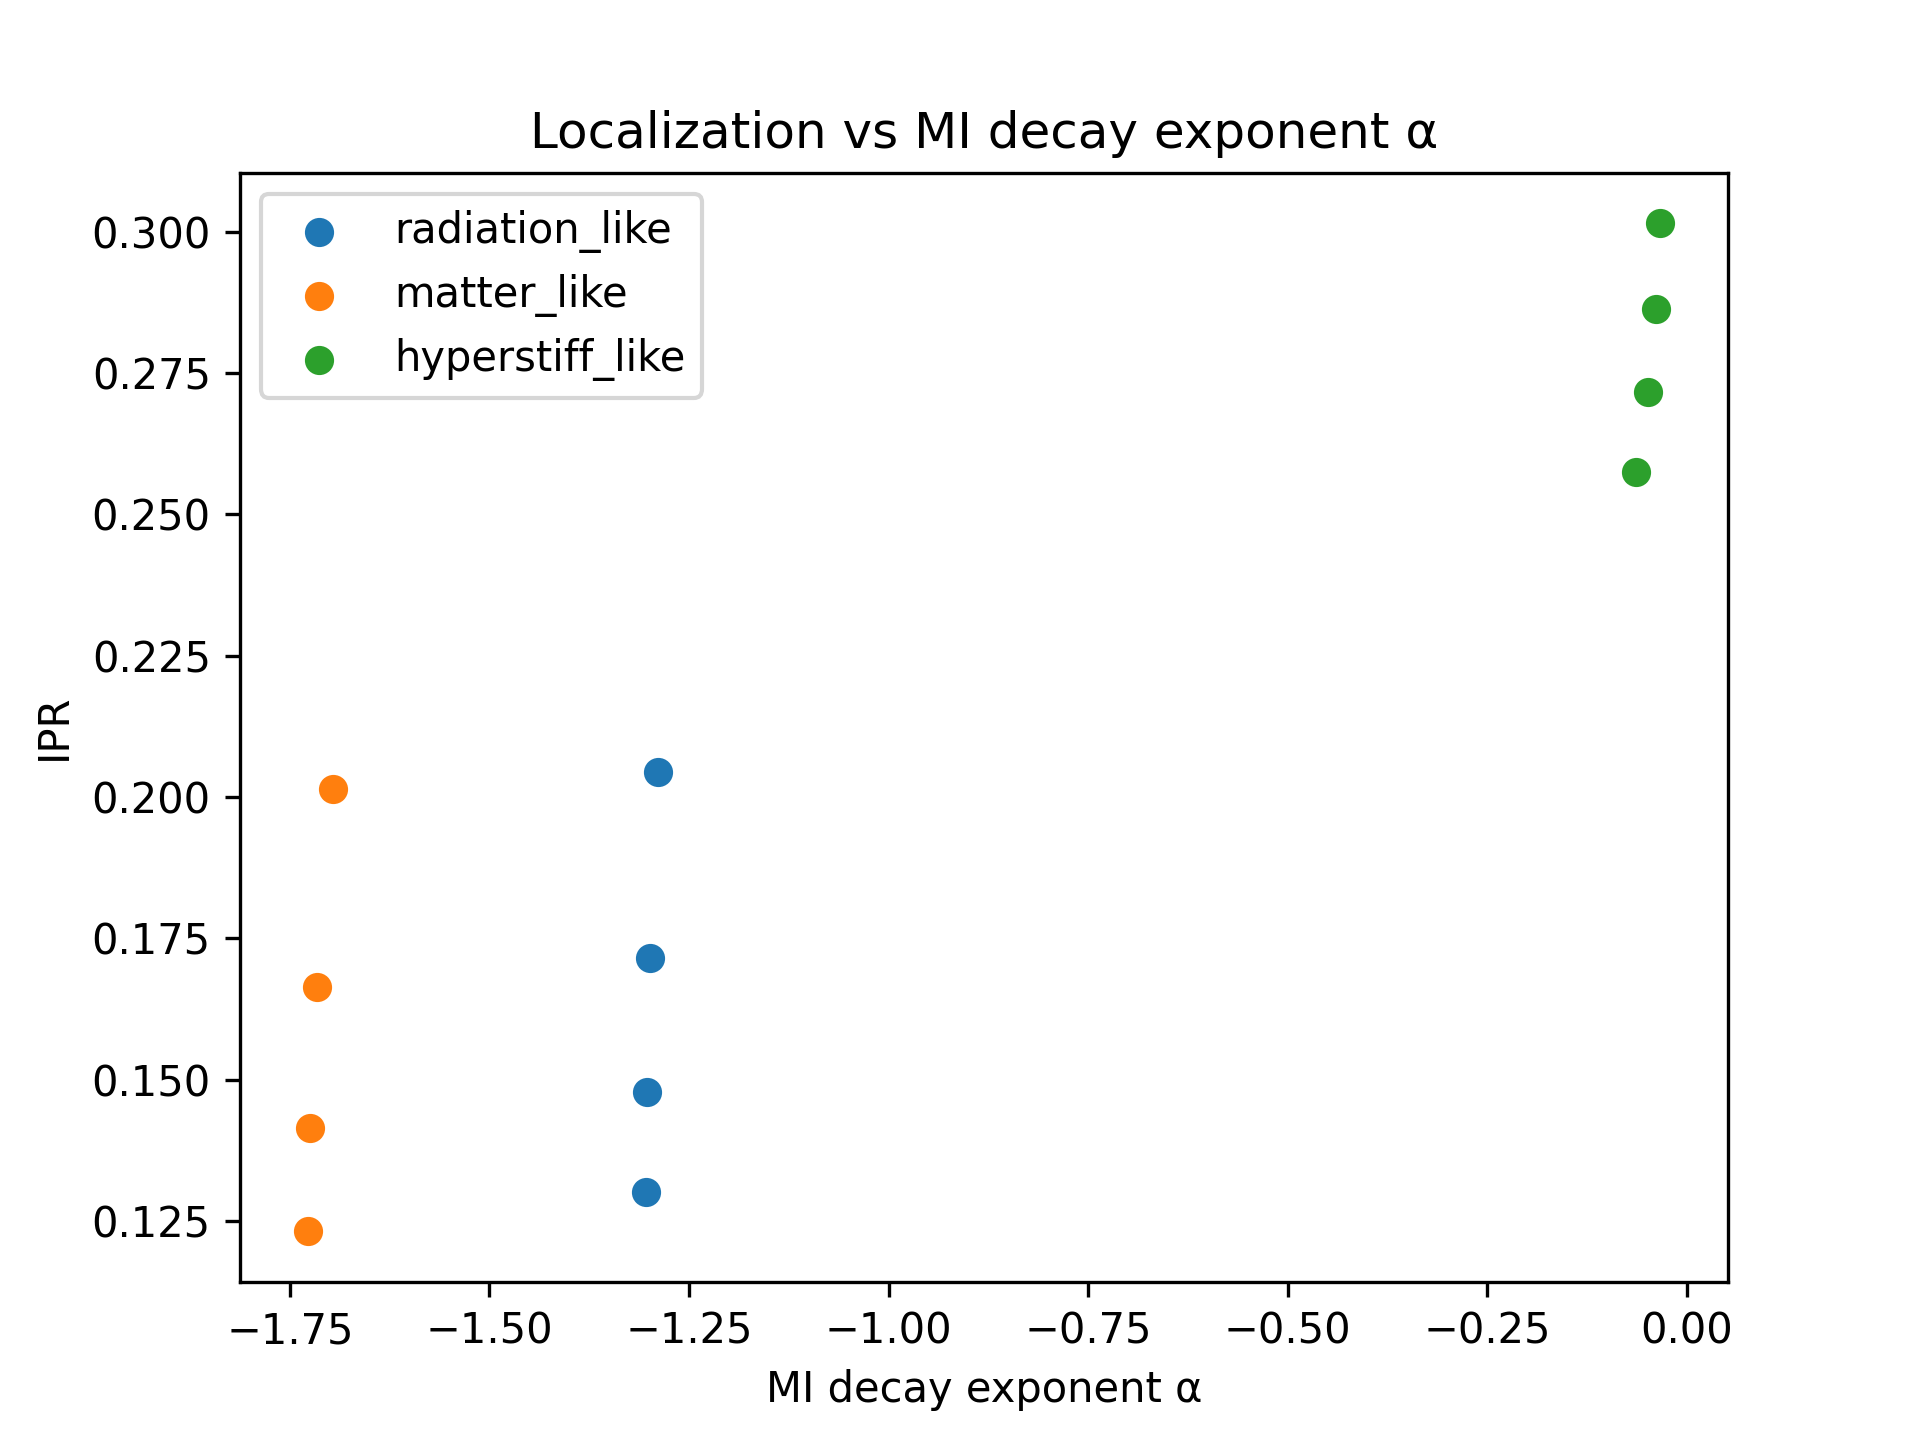
\includegraphics[width=0.8\textwidth]{FIG10_alpha_vs_lam1.png}
\caption{Localization vs.\ MI decay exponent $\alpha$.}
\label{fig:IPRvsAlpha}
\end{figure}

\section{Discussion}

The combined results reveal a new physical correspondence:

\begin{center}
\begin{tabular}{|c|c|}
\hline
Cosmological Phase & Entanglement-Geometric Signature \\
\hline
Radiation ($w=1/3$) & Critical, extended geometry \\
Matter ($w=0$) & Weakly gapped geometry \\
Hyper-stiff ($w \gg 1$) & Strongly gapped, ultra-dense geometry \\
\hline
\end{tabular}
\end{center}

This dictionary suggests that:

\begin{itemize}
    \item The hyper-stiff spike in brane-rupture cosmology corresponds to a mass-gap explosion in entanglement geometry.
    \item The millihertz turnover in the gravitational-wave spectrum corresponds to a Laplacian spectral cutoff.
    \item The early-time sound-horizon reduction corresponds to a suppression of correlation length.
    \item Early-universe topology change may be encoded directly in the structure of quantum correlations.
\end{itemize}

\subsection*{Finite-size limitations}

Exact diagonalization restricts us to $N \leq 14$, but the phase separation is already robust across this range.  
Radiation-like and matter-like phases show monotonic decay of $\lambda_1$ with $1/N^2$, while hyper-stiff analogues show monotonic growth.  
Bootstrap and null-model tests confirm that these trends are not finite-size artifacts.  
Larger-$N$ simulations (DMRG or tensor networks) are a natural extension but are not required to establish the entanglement--cosmology dictionary.

\section{Conclusion}

We have shown that hyper-stiff cosmological phases---arising naturally from brane rupture and confinement-energy release---have a precise analogue in entanglement geometry: they correspond to strongly gapped, ultra-dense geometries with rapidly increasing mass scale. This connection unifies three previously independent results and opens a new direction in which early-universe physics can be probed through quantum-information diagnostics.

\end{document}
